\begin{tikzpicture}[node distance=4.5cm,thick,auto,main node/.style={rectangle,draw}]
    \node[main node] (1) {Plano $z$};
    \node[main node] (2) [below of=1] {Plano $\gamma$};
    \node[main node] (3) [right of=2] {Plano $\tau$};
    \node[main node] (4) [right of=3] {Plano $\lambda$};
    \node[main node] (5) [above of=4] {Plano $w$};
    \path[every node/.style={font=\sffamily\small}];
    \draw[-latex]
    (1) edge  node {Traslación $z_1$} (2)
        edge  node {$F_{(z)=}z_0+\kappa\cfrac{1}{z+z_1}$} (5)
    (2) edge  node {Reciproca $\frac{1}{z}$} (3)
    (3) edge  node {Escalado $\kappa$} (4)
    (4) edge  node[right] {Traslación $z_0$} (5);
\end{tikzpicture}